\documentclass[14pt]{extbook}
\usepackage{multicol, enumerate, enumitem, hyperref, color, soul, setspace, parskip, fancyhdr} %General Packages
\usepackage{amssymb, amsthm, amsmath, latexsym, units, mathtools} %Math Packages
\everymath{\displaystyle} %All math in Display Style
% Packages with additional options
\usepackage[headsep=0.5cm,headheight=12pt, left=1 in,right= 1 in,top= 1 in,bottom= 1 in]{geometry}
\usepackage[usenames,dvipsnames]{xcolor}
\usepackage{dashrule}  % Package to use the command below to create lines between items
\newcommand{\litem}[1]{\item#1\hspace*{-1cm}\rule{\textwidth}{0.4pt}}
\pagestyle{fancy}
\lhead{Progress Quiz 7}
\chead{}
\rhead{Version A}
\lfoot{6523-2736}
\cfoot{}
\rfoot{test}
\begin{document}

\begin{enumerate}
\litem{
Solve the quadratic equation below. Then, choose the intervals that the solutions belong to, with $x_1 \leq x_2$ (if they exist).\[ 13x^{2} +10 x -4 = 0 \]\begin{enumerate}[label=\Alph*.]
\item \( x_1 \in [-1, -0.28] \text{ and } x_2 \in [0.6, 2.8] \)
\item \( x_1 \in [-18.81, -17.81] \text{ and } x_2 \in [16.2, 18.8] \)
\item \( x_1 \in [-2.04, -0.73] \text{ and } x_2 \in [0.1, 0.5] \)
\item \( x_1 \in [-14.09, -13.48] \text{ and } x_2 \in [2.3, 3.9] \)
\item \( \text{There are no Real solutions.} \)

\end{enumerate} }
\litem{
Solve the quadratic equation below. Then, choose the intervals that the solutions belong to, with $x_1 \leq x_2$ (if they exist).\[ -20x^{2} -14 x + 2 = 0 \]\begin{enumerate}[label=\Alph*.]
\item \( x_1 \in [-1.4, -0.76] \text{ and } x_2 \in [-0.54, 0.36] \)
\item \( x_1 \in [-2.47, -2.41] \text{ and } x_2 \in [16.27, 17.01] \)
\item \( x_1 \in [-19.95, -18.57] \text{ and } x_2 \in [18.46, 18.56] \)
\item \( x_1 \in [-0.56, 0.93] \text{ and } x_2 \in [0.64, 1.12] \)
\item \( \text{There are no Real solutions.} \)

\end{enumerate} }
\litem{
Solve the quadratic equation below. Then, choose the intervals that the solutions $x_1$ and $x_2$ belong to, with $x_1 \leq x_2$.\[ 25x^{2} -50 x + 24 = 0 \]\begin{enumerate}[label=\Alph*.]
\item \( x_1 \in [19.86, 20.01] \text{ and } x_2 \in [29.85, 30.14] \)
\item \( x_1 \in [0.4, 0.45] \text{ and } x_2 \in [2.16, 2.89] \)
\item \( x_1 \in [0.51, 0.63] \text{ and } x_2 \in [1.41, 2.02] \)
\item \( x_1 \in [0.21, 0.38] \text{ and } x_2 \in [3.68, 4.15] \)
\item \( x_1 \in [0.75, 0.86] \text{ and } x_2 \in [1.07, 1.44] \)

\end{enumerate} }
\litem{
Graph the equation below.\[ f(x) = (x-2)^2 - 12 \]\begin{enumerate}[label=\Alph*.]
\begin{multicols}{2}\item 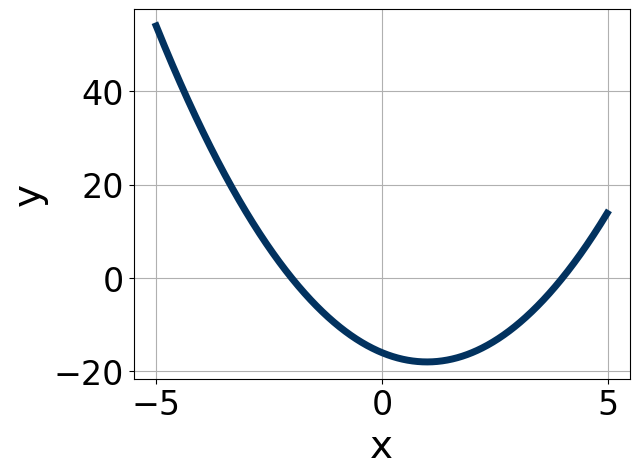
\includegraphics[width = 0.3\textwidth]{../Figures/quadraticEquationToGraphAA.png}\item 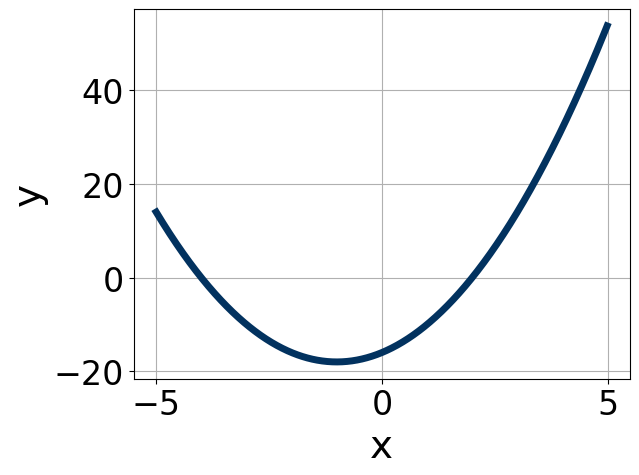
\includegraphics[width = 0.3\textwidth]{../Figures/quadraticEquationToGraphBA.png}\item 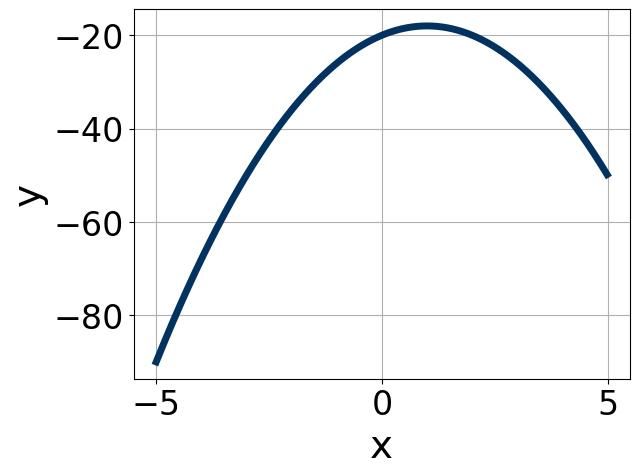
\includegraphics[width = 0.3\textwidth]{../Figures/quadraticEquationToGraphCA.png}\item 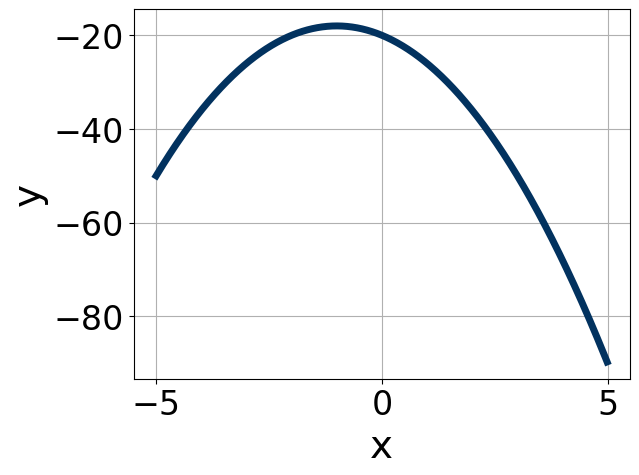
\includegraphics[width = 0.3\textwidth]{../Figures/quadraticEquationToGraphDA.png}\end{multicols}\item None of the above.
\end{enumerate} }
\litem{
Factor the quadratic below. Then, choose the intervals that contain the constants in the form $(ax+b)(cx+d); b \leq d.$\[ 36x^{2} +60 x + 25 \]\begin{enumerate}[label=\Alph*.]
\item \( a \in [11.9, 13.4], \hspace*{5mm} b \in [2, 11], \hspace*{5mm} c \in [1.1, 3.6], \text{ and } \hspace*{5mm} d \in [5, 7] \)
\item \( a \in [0.6, 2.4], \hspace*{5mm} b \in [24, 40], \hspace*{5mm} c \in [-1.7, 2.9], \text{ and } \hspace*{5mm} d \in [30, 35] \)
\item \( a \in [2.8, 4.5], \hspace*{5mm} b \in [2, 11], \hspace*{5mm} c \in [9, 13.2], \text{ and } \hspace*{5mm} d \in [5, 7] \)
\item \( a \in [4, 6.2], \hspace*{5mm} b \in [2, 11], \hspace*{5mm} c \in [5.5, 8.6], \text{ and } \hspace*{5mm} d \in [5, 7] \)
\item \( \text{None of the above.} \)

\end{enumerate} }
\litem{
Factor the quadratic below. Then, choose the intervals that contain the constants in the form $(ax+b)(cx+d); b \leq d.$\[ 24x^{2} -38 x + 15 \]\begin{enumerate}[label=\Alph*.]
\item \( a \in [3.9, 6.1], \hspace*{5mm} b \in [-9, -3], \hspace*{5mm} c \in [2.8, 5.08], \text{ and } \hspace*{5mm} d \in [-3, 3] \)
\item \( a \in [1.3, 4], \hspace*{5mm} b \in [-9, -3], \hspace*{5mm} c \in [6.61, 8.68], \text{ and } \hspace*{5mm} d \in [-3, 3] \)
\item \( a \in [-1.4, 2.1], \hspace*{5mm} b \in [-24, -18], \hspace*{5mm} c \in [-0.37, 1.63], \text{ and } \hspace*{5mm} d \in [-19, -15] \)
\item \( a \in [7.4, 12.2], \hspace*{5mm} b \in [-9, -3], \hspace*{5mm} c \in [1.72, 2.76], \text{ and } \hspace*{5mm} d \in [-3, 3] \)
\item \( \text{None of the above.} \)

\end{enumerate} }
\litem{
Graph the equation below.\[ f(x) = (x+4)^2 - 15 \]\begin{enumerate}[label=\Alph*.]
\begin{multicols}{2}\item 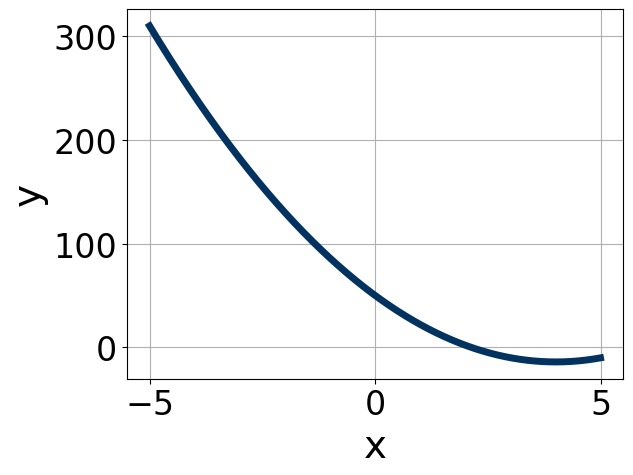
\includegraphics[width = 0.3\textwidth]{../Figures/quadraticEquationToGraphCopyAA.png}\item 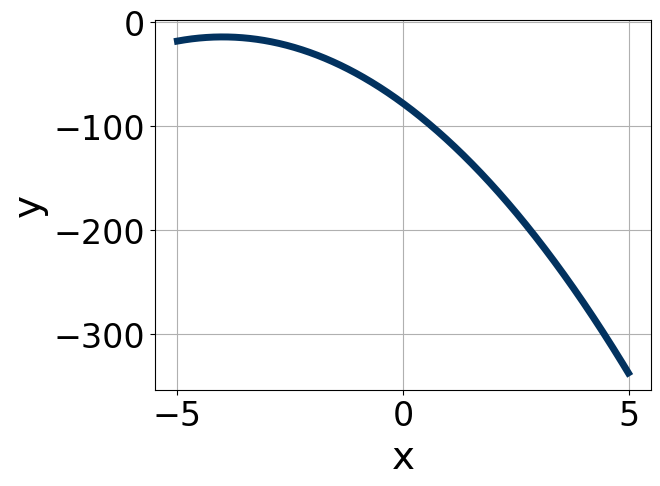
\includegraphics[width = 0.3\textwidth]{../Figures/quadraticEquationToGraphCopyBA.png}\item 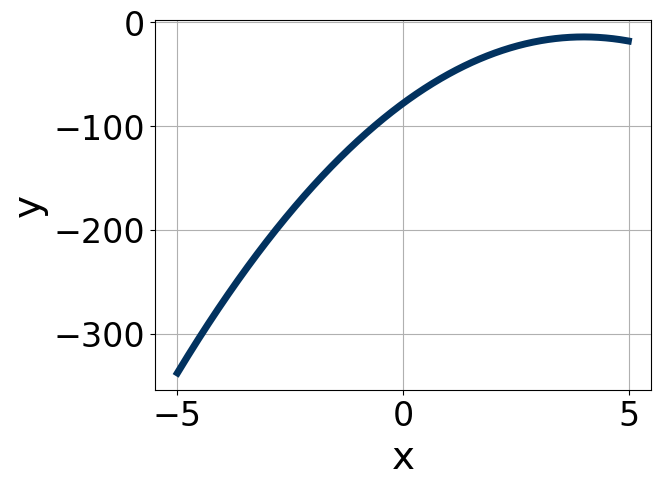
\includegraphics[width = 0.3\textwidth]{../Figures/quadraticEquationToGraphCopyCA.png}\item 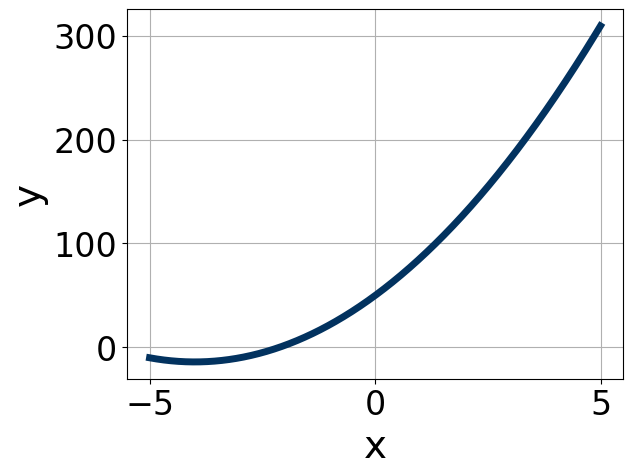
\includegraphics[width = 0.3\textwidth]{../Figures/quadraticEquationToGraphCopyDA.png}\end{multicols}\item None of the above.
\end{enumerate} }
\litem{
Solve the quadratic equation below. Then, choose the intervals that the solutions $x_1$ and $x_2$ belong to, with $x_1 \leq x_2$.\[ 20x^{2} +21 x -54 = 0 \]\begin{enumerate}[label=\Alph*.]
\item \( x_1 \in [-10.23, -8.78] \text{ and } x_2 \in [0.1, 0.37] \)
\item \( x_1 \in [-45.23, -44.45] \text{ and } x_2 \in [23.88, 24.04] \)
\item \( x_1 \in [-4.41, -1.2] \text{ and } x_2 \in [1.11, 1.36] \)
\item \( x_1 \in [-7.7, -6.16] \text{ and } x_2 \in [0.39, 0.43] \)
\item \( x_1 \in [-1.4, 0.74] \text{ and } x_2 \in [2.36, 2.49] \)

\end{enumerate} }
\litem{
Write the equation of the graph presented below in the form $f(x)=ax^2+bx+c$, assuming  $a=1$ or $a=-1$. Then, choose the intervals that $a, b,$ and $c$ belong to.
\begin{center}
    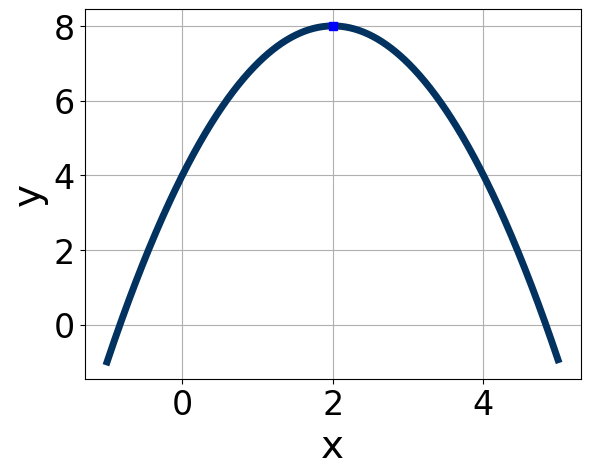
\includegraphics[width=0.5\textwidth]{../Figures/quadraticGraphToEquationCopyA.png}
\end{center}
\begin{enumerate}[label=\Alph*.]
\item \( a \in [-2.6, -0.2], \hspace*{5mm} b \in [-9, -4], \text{ and } \hspace*{5mm} c \in [-8, -5] \)
\item \( a \in [-2.6, -0.2], \hspace*{5mm} b \in [8, 9], \text{ and } \hspace*{5mm} c \in [-8, -5] \)
\item \( a \in [0.7, 3.3], \hspace*{5mm} b \in [-9, -4], \text{ and } \hspace*{5mm} c \in [26, 28] \)
\item \( a \in [0.7, 3.3], \hspace*{5mm} b \in [8, 9], \text{ and } \hspace*{5mm} c \in [26, 28] \)
\item \( a \in [-2.6, -0.2], \hspace*{5mm} b \in [8, 9], \text{ and } \hspace*{5mm} c \in [-26, -24] \)

\end{enumerate} }
\litem{
Write the equation of the graph presented below in the form $f(x)=ax^2+bx+c$, assuming  $a=1$ or $a=-1$. Then, choose the intervals that $a, b,$ and $c$ belong to.
\begin{center}
    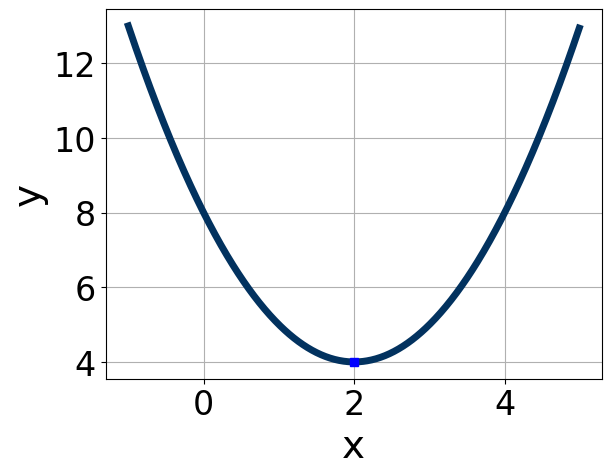
\includegraphics[width=0.5\textwidth]{../Figures/quadraticGraphToEquationA.png}
\end{center}
\begin{enumerate}[label=\Alph*.]
\item \( a \in [-1.6, 0], \hspace*{5mm} b \in [-10, -6], \text{ and } \hspace*{5mm} c \in [-8, -6] \)
\item \( a \in [-1.6, 0], \hspace*{5mm} b \in [-10, -6], \text{ and } \hspace*{5mm} c \in [-24, -21] \)
\item \( a \in [-1.6, 0], \hspace*{5mm} b \in [8, 11], \text{ and } \hspace*{5mm} c \in [-8, -6] \)
\item \( a \in [-0.8, 2.1], \hspace*{5mm} b \in [8, 11], \text{ and } \hspace*{5mm} c \in [22, 25] \)
\item \( a \in [-0.8, 2.1], \hspace*{5mm} b \in [-10, -6], \text{ and } \hspace*{5mm} c \in [22, 25] \)

\end{enumerate} }
\end{enumerate}

\end{document}